

\tikzset{every picture/.style={line width=0.5pt}} %set default line width to 0.75pt        

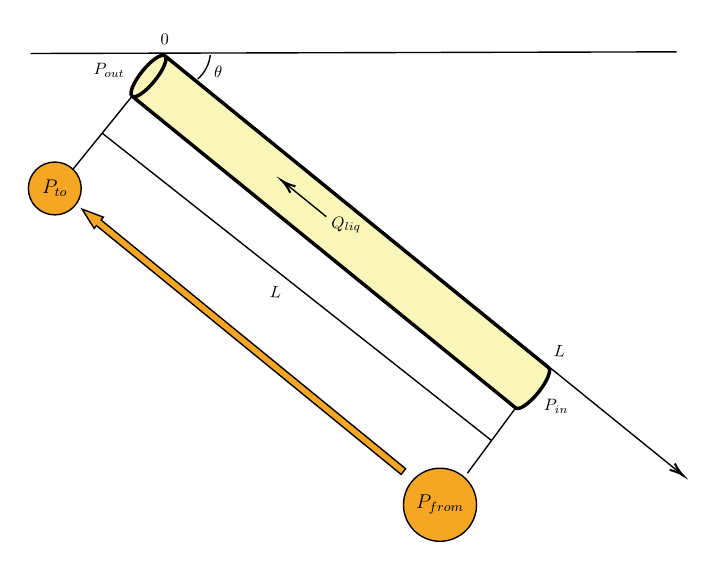
\begin{tikzpicture}[x=0.75pt,y=0.75pt, yscale=-0.6, xscale=0.6, every node/.style={scale=0.6}]
%uncomment if require: \path (0,436); %set diagram left start at 0, and has height of 436

%Right Arrow [id:dp23899496640302043] 
\draw  [fill={rgb, 255:red, 245; green, 166; blue, 35 }  ,fill opacity=1 ] (393.73,367.97) -- (149.14,168.2) -- (147.29,170.47) -- (137.56,154.96) -- (154.7,161.41) -- (152.84,163.67) -- (397.43,363.44) -- cycle ;
%Shape: Can [id:dp3614373882368076] 
\draw  [fill={rgb, 255:red, 250; green, 245; blue, 184 }  ,fill opacity=1 ][line width=1.25]  (204.09,31.86) -- (512.1,282.18) .. controls (514.79,284.36) and (511.07,293.39) .. (503.8,302.34) .. controls (496.52,311.29) and (488.45,316.77) .. (485.76,314.59) -- (177.75,64.28) .. controls (175.07,62.09) and (178.79,53.07) .. (186.06,44.12) .. controls (193.33,35.17) and (201.41,29.68) .. (204.09,31.86) .. controls (206.78,34.05) and (203.06,43.07) .. (195.78,52.02) .. controls (188.51,60.97) and (180.44,66.46) .. (177.75,64.28) ;
%Shape: Arc [id:dp28101757111719494] 
\draw  [draw opacity=0] (240.53,31.24) .. controls (240.15,34.58) and (239.2,37.91) .. (237.64,41.1) .. controls (235.82,44.8) and (233.34,47.95) .. (230.42,50.5) -- (210.71,27.87) -- cycle ; \draw   (240.53,31.24) .. controls (240.15,34.58) and (239.2,37.91) .. (237.64,41.1) .. controls (235.82,44.8) and (233.34,47.95) .. (230.42,50.5) ;
%Straight Lines [id:da01226354778251526] 
\draw    (177.75,64.28) -- (129.67,123.67) ;
%Straight Lines [id:da5968116354705983] 
\draw    (485.76,314.59) -- (447,367) ;
%Straight Lines [id:da1296308910316466] 
\draw    (153.71,93.97) -- (466.38,340.8) ;
%Straight Lines [id:da9143934640782487] 
\draw    (333.67,161) -- (299.89,133.6) ;
\draw [shift={(298.33,132.34)}, rotate = 399.05] [color={rgb, 255:red, 0; green, 0; blue, 0 }  ][line width=0.75]    (10.93,-3.29) .. controls (6.95,-1.4) and (3.31,-0.3) .. (0,0) .. controls (3.31,0.3) and (6.95,1.4) .. (10.93,3.29)   ;
%Straight Lines [id:da5765585120025118] 
\draw    (96.33,30) -- (615,28.67) ;
%Straight Lines [id:da7775845222697451] 
\draw    (204.09,31.86) -- (618.45,367.41) ;
\draw [shift={(620,368.67)}, rotate = 219] [color={rgb, 255:red, 0; green, 0; blue, 0 }  ][line width=0.75]    (10.93,-3.29) .. controls (6.95,-1.4) and (3.31,-0.3) .. (0,0) .. controls (3.31,0.3) and (6.95,1.4) .. (10.93,3.29)   ;

% Text Node
\draw  [color={rgb, 255:red, 0; green, 0; blue, 0 }  ,draw opacity=1 ][fill={rgb, 255:red, 245; green, 166; blue, 35 }  ,fill opacity=1 ]  (425, 392.37) circle [x radius= 29.33, y radius= 29.33]   ;
\draw (425,392.37) node  [font=\large,rotate=-359.71]  {$P_{from}$};
% Text Node
\draw  [fill={rgb, 255:red, 245; green, 166; blue, 35 }  ,fill opacity=1 ]  (115.67, 138.37) circle [x radius= 21.22, y radius= 21.22]   ;
\draw (115.67,138.37) node  [font=\large,rotate=-0.74]  {$P_{to}$};
% Text Node
\draw (247,44.67) node    {$\theta $};
% Text Node
\draw (293,221.33) node  [rotate=-2.44]  {$L$};
% Text Node
\draw (518.33,313.33) node  [rotate=-0.74]  {$P_{in}$};
% Text Node
\draw (159.33,43.67) node  [rotate=-0.74]  {$P_{out}$};
% Text Node
\draw (349.67,167.67) node  [rotate=-0.61]  {$Q_{liq}$};
% Text Node
\draw (204,18.33) node  [rotate=-2.44]  {$0$};
% Text Node
\draw (521,269.33) node  [rotate=-2.44]  {$L$};


\end{tikzpicture}